\documentclass{beamer}

\usepackage[czech]{babel}
\usepackage[utf8]{inputenc}
%\usepackage[plainpages=false,pdfpagelabels,unicode]{hyperref}
\usepackage{graphicx}

\usetheme{Warsaw}

\begin{document}

\title[Optical properties of dioxides by first principle calculations] % (optional, only for long titles)
{Optical properties of various dioxides by first principle calculations}
\subtitle{The road so far...}
\author{Pavel Ondračka}
\institute
{
	 Faculty of Science, Masaryk University\\
	Brno, Czech Republic
  \and
	CEITEC - Central European Institute of Technology\\
	Brno, Czech Republic
}
\date{29.10.2014}

\maketitle

\begin{frame}
	\frametitle{Outline}
    \tableofcontents
\end{frame}

\section{Motivation}
\begin{frame}
    \frametitle{Motivation}
    \framesubtitle{We want to calculate everything!}
	In theory we could use DFT calculations to:
	\begin{itemize}	
	\item calculate optical properties in broad spectral range (including core electron excitations)
	\item predict optical properties of new materials
	\item better understand underlying processes
	\item help development of new dispersion models
	\end{itemize}
\end{frame}

\section{Introduction}
\subsection{DFT}
\begin{frame}
    \frametitle{DFT introduction}
    \framesubtitle{It shoudl be easy? Right?}

	Hohenberg–Kohn theorems:
	\begin{itemize}
	\item The ground state properties of a many-electron system are uniquely determined by an electron density that depends on only 3 spatial coordinates.
	\item The second theorem defines an energy functional for the system and proves that the correct ground state electron density minimizes this energy functional.
	\end{itemize}
	So we can reduce the many-body problem of $N$ electrons with $3N$ spatial coordinates to 3 spatial coordinates.
\end{frame}

\begin{frame}
    \frametitle{DFT introduction}
    \framesubtitle{Not so easy after all...}

	\begin{itemize}
	\item Born–Oppenheimer approximation.
	\item $\hat{H} = \hat{V} + \hat{T} + \hat{U}$
	\item external potential $\hat{V}$ is system-dependent, kinetic energy $\hat{T}$ and electron-electron interaction energy $\hat{U}$ are not
	\item $E_0 = E[n_0] = <\Psi[n_0] | \hat{H} | \Psi[n_0]> $
	\item $[-\frac{\hbar}{2m} \nabla^2 + V_\mathrm{s} ] \phi_i(\vec{r}) = \epsilon_i \phi_i(\vec{r}) $
	\item $n(\vec{r}) = \sum_i^N | \phi_i(\vec{r}) |^2$
	\item $V_\mathrm{s}(\vec{r}) = V(\vec{r}) + \int{\frac{e^2 n_\mathrm{s}(\vec{r}')}{|\vec{r}-\vec{r}'|d^3r'}} + V_\mathrm{xc}[n_\mathrm{s}(\vec{r})]$
	\item exact form of $V_\mathrm{xc}[n_\mathrm{s}(\vec{r})]$ unknown (LDA, GGA etc.)

	\end{itemize}

\end{frame}

\begin{frame}
    \frametitle{Wien2k}
%    \framesubtitle{}

	\begin{itemize}
	\item All electron full potential fully relativistic DFT code 
	\item LAPW basis
	\item quite cheap licence
	\item included optic package for calculation of optical properties
	\item runs on UNIX and supports heavy parallelisation (k-point, MPI)
	\item in theory the only input needed is the external potential (e.g. unit cell of the material), however due to numerical calculations you need to tweak a LOT of other parameters to reach convergence
	\item periodic boundary condition

	\end{itemize}

\end{frame}

\subsection{Optics}
\begin{frame}
    \frametitle{Selected optical definitions}
    \framesubtitle{What all those letters stand for?}

	There are few terms to describe optical response

	\begin{itemize}
	\item Refractive index $n$ and extinction coefficient $\kappa$, sometimes called complex refractive index $\tilde{n} = n + \mathrm{i} \kappa$
	\item Complex dielectric function $\tilde{\epsilon} = \epsilon_\mathrm{r} + \epsilon_\mathrm{i}$, or for nonisotropic materials dielectric tensor $\hat{\epsilon}$.
	\item $\epsilon_\mathrm{r} = n^2 - \kappa^2 $, $\epsilon_\mathrm{i} = 2 n \kappa$
	\item Absorption (attenuation) coefficient $\alpha = \frac{4 \pi \kappa}{\lambda}$ as known from Beer-Lambert law $I = I_0 \mathrm{e}^{-\alpha x}$  
	\end{itemize} 
	\small
	\begin{equation}	
	\epsilon_\mathrm{i} (E) = 
\left(\frac{eh}{m_\mathrm{e}E} \right)^2 \frac{1}{4 \pi \epsilon_0 \mathrm{B}_0} \sum_{j,k} | p_{j \rightarrow k} |^2
\int_{-\infty}^\infty f_\mathrm{e}(S) \mathcal{N}_j(S) f_\mathrm{h}(S+E) \mathcal{N}_k(S + E)\mathrm{d}S \text{,}
	\end{equation}
	\normalsize
\end{frame}

\begin{frame}
    \frametitle{Selected optical definitions}
    \framesubtitle{No more equations, I promise}

Kramers-Kronig relations:
\begin{equation}
\epsilon_\mathrm{r}(\omega) = 1 + \frac{1}{\pi} \mathcal{P} \int \frac{\epsilon_\mathrm{i}(\xi)}{\xi - \omega} \mathrm{d}\xi \mathrm{,}
\label{KKint}
\end{equation}

So called optical sum rule:
\begin{equation}
\int_0^\infty \epsilon_\mathrm{i} (\omega) \omega \mathrm{d} \omega = \frac{\pi}{2} \omega_\mathrm{p}^2 = \frac{\pi}{2} \frac{e^2 n_\mathrm{e}}{ \epsilon_0 m_\mathrm{e}} \mathrm{,}
\end{equation}

\end{frame}

\section{Selected problems}
\subsection{Correct band gap}

\begin{frame}
    \frametitle{Correct band gap}
    \framesubtitle{Its all about the potential}

	DFT is known to underestimate the band gap.

	Possible solutions:
	\begin{itemize}
	\item scissor operator (no additional computational cost)
	\item orbital potential (LDA+U, GGA+U) (same order as LDA or GGA)
	\item mBJ exchange-correlation potential (same order as LDA or GGA)
	\item hybrid potential (expensive)
	\item GW (expensive)
	\end{itemize}
\end{frame}

\begin{frame}
    \frametitle{Correct band gap}
    \framesubtitle{mBJ seems to be the best solution}

    \begin{figure}
	\includegraphics[width=0.8\linewidth]{figures/compare.pdf}
	\end{figure}

\end{frame}

\begin{frame}
    \frametitle{Correct band gap}
    \framesubtitle{Correct band gap comes at cost}
	TiO$_2$ rutile band structure
	\begin{figure}
	\hspace{0.2cm} GGA \hspace{2.4cm} mBJ \hspace{2.8cm} G$_0$W$_0$\footnote{M Landmann, E Rauls, and W G Schmidt. Journal of Physics: Condensed Matter, 24(19):195503, 2012.}
	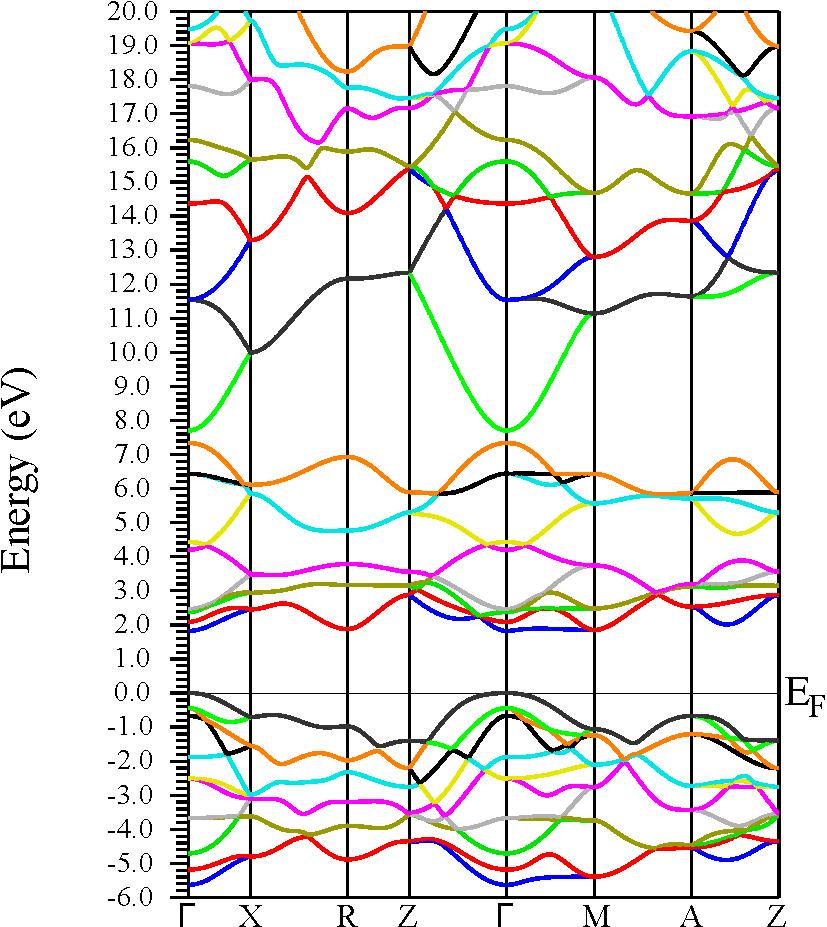
\includegraphics[height=3.8cm]{figures/TiO2-rutile-GGA.pdf}
	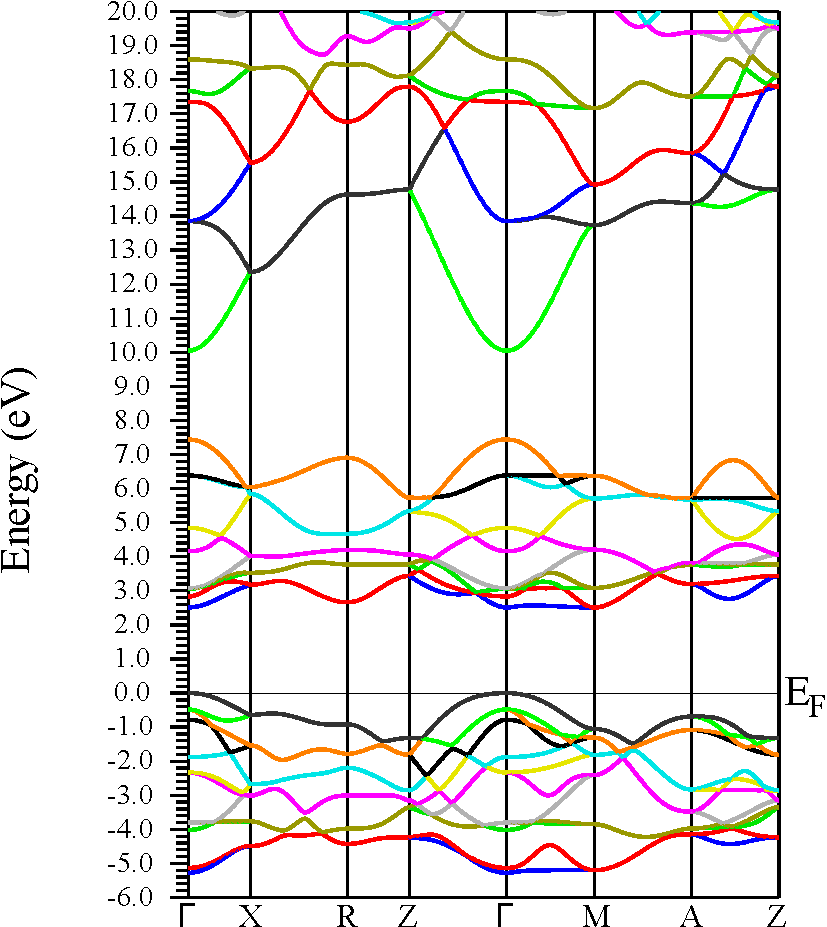
\includegraphics[height=3.8cm]{figures/TiO2-rutile-mBJ.pdf}
	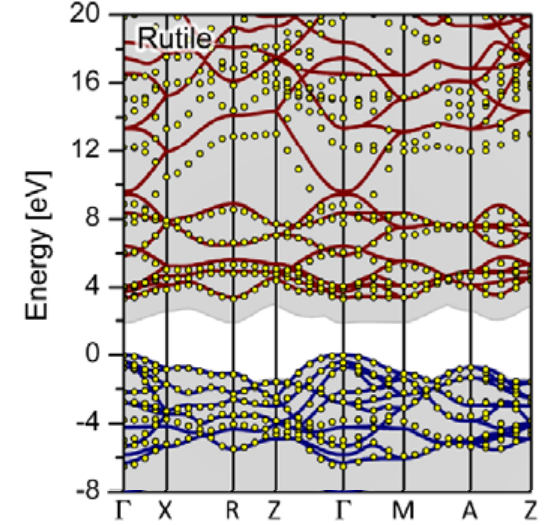
\includegraphics[height=3.8cm]{figures/TiO2-rutile-GW.png}
	\end{figure}

\end{frame}

\subsection{Dielectric function in wide spectral range}
\begin{frame}
    \frametitle{Dielectric function in wide spectral range}
    \framesubtitle{Why is is important?}

	\begin{itemize}
	\item Advanced dispersion models can provide information such as mass density
	\item But we need information from outside spectral range of usual optical measurements 
	\item Also estimation of effective number of electrons is needed 
	\item DFT results could be used to enhance current (mostly empirical) models
	\end{itemize}	

\end{frame}

\begin{frame}
    \frametitle{Dielectric function in wide spectral range}
    \framesubtitle{HfO$_2$ example}

    \begin{figure}
	\includegraphics[width=\linewidth]{figures/HfO2-eps-overview.pdf}
	\end{figure}

\end{frame}

\subsection{Understanding the nature of electronic transitions}
\begin{frame}
    \frametitle{Understanding nature of electronic transitions}
    \framesubtitle{Another way to enhance dispersion models}

	\begin{columns}[c]
    \column{.4\textwidth}
	As was shown in (1), dielectric function is constructed by summing over all possible electron transitions, hence we can use this information to analyze them and reveal different transition types

    \column{.6\textwidth}
    \begin{figure}
	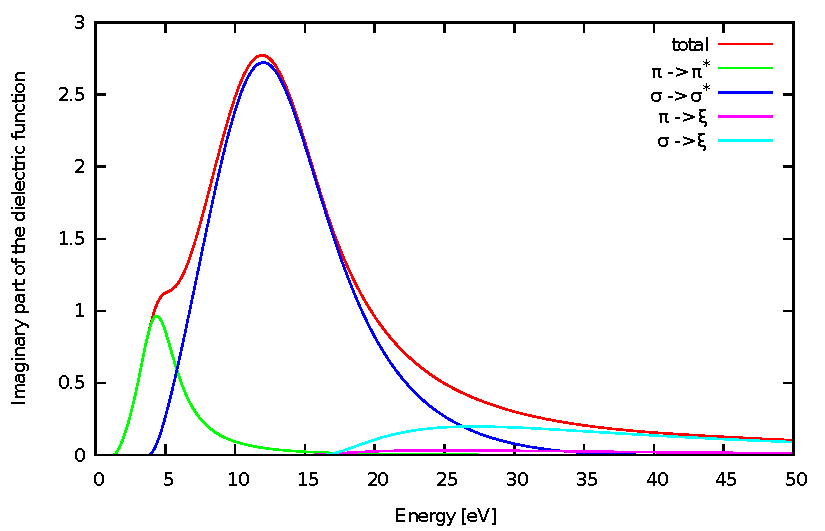
\includegraphics[width=\linewidth]{figures/CH30deconv.pdf}
	\end{figure}
	\end{columns}

\end{frame}

\begin{frame}
    \frametitle{Understanding nature of electronic transitions}
    \framesubtitle{Divide and conquer}

	\begin{columns}[c]
    \column{.8\textwidth}
	\vspace{-0.5cm}

    \begin{figure}
	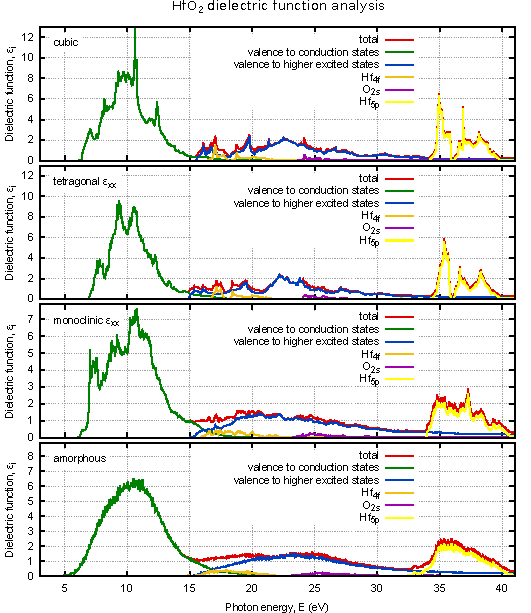
\includegraphics[height=6.8cm]{figures/cubic-eps.pdf}
	\end{figure}

    \column{.2\textwidth}
	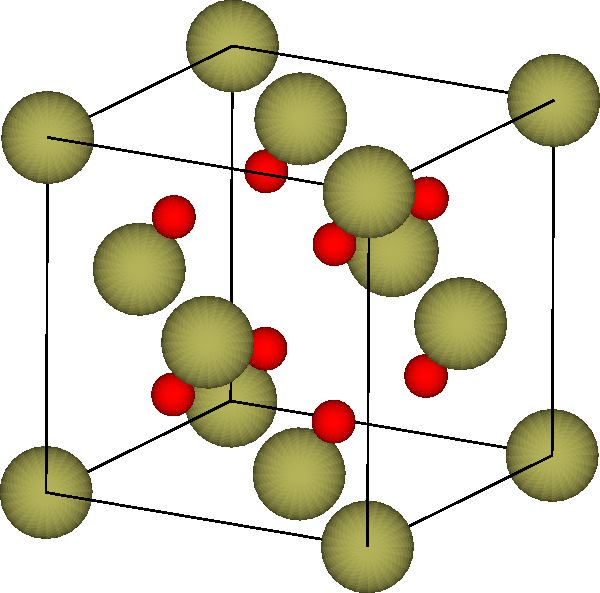
\includegraphics[width=0.75\linewidth]{figures/cubic.pdf}

	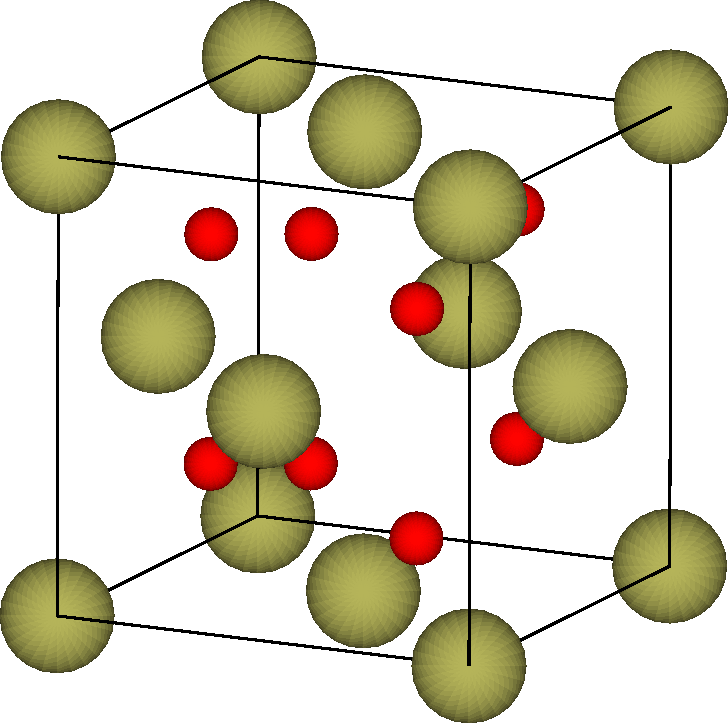
\includegraphics[width=0.75\linewidth]{figures/tetragonal.pdf}

	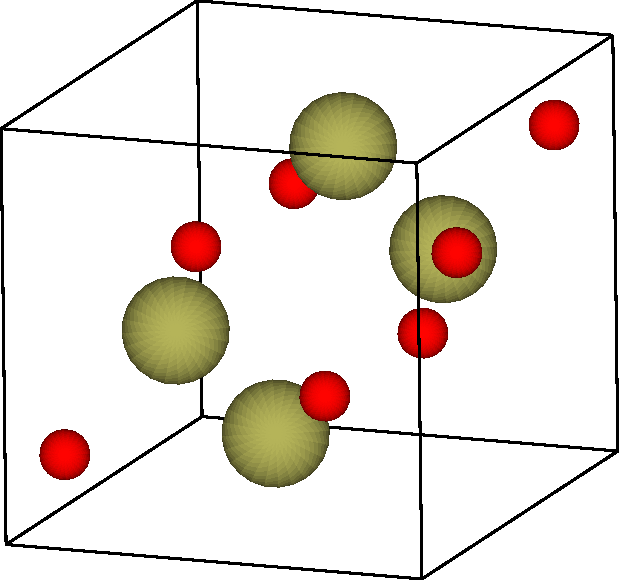
\includegraphics[width=0.75\linewidth]{figures/monoclinic.pdf}

	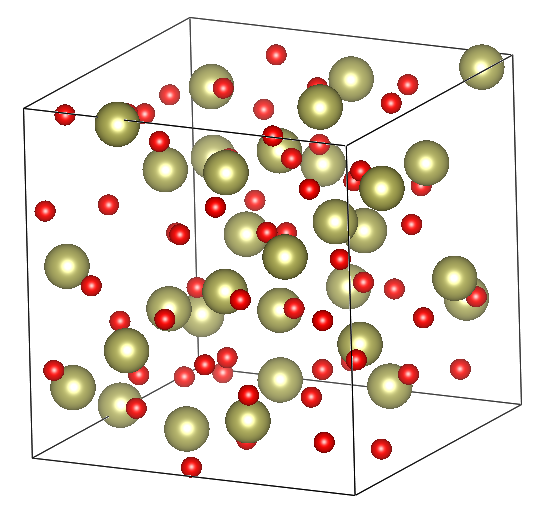
\includegraphics[width=0.75\linewidth]{figures/am.png}
    \end{columns}

\end{frame}

\subsection{Predictions of new materials}
\begin{frame}
    \frametitle{Predictions of new materials - Si$_x$Ti$_{1-x}$O$_2$}
    \framesubtitle{As long as its periodic, we can calculate it}

	\begin{columns}[c]
    \column{.5\textwidth}
     TiO$_2$-SiO$_2$ materials are very promising for optical applications, we used DFT to model Si$_x$Ti$_{1-x}$O$_2$ solid solutions for various $x$ values

    \begin{figure}
	\includegraphics[width=\linewidth]{figures/gap.pdf}
	\end{figure}
    \column{.5\textwidth}

    \begin{figure}
	\includegraphics[width=\linewidth]{figures/SiTiO2-eps.pdf}
	\end{figure}

    \end{columns}
\end{frame}


\begin{frame}
    \frametitle{Predictions of new materials - Si$_x$Ti$_{1-x}$O$_2$}
    \framesubtitle{Some interesting behavior showed up}

	\begin{columns}[c]
    \column{.4\textwidth}

    \begin{figure}
	\includegraphics[width=\linewidth]{figures/near-gap-eps.pdf}
	\newline
	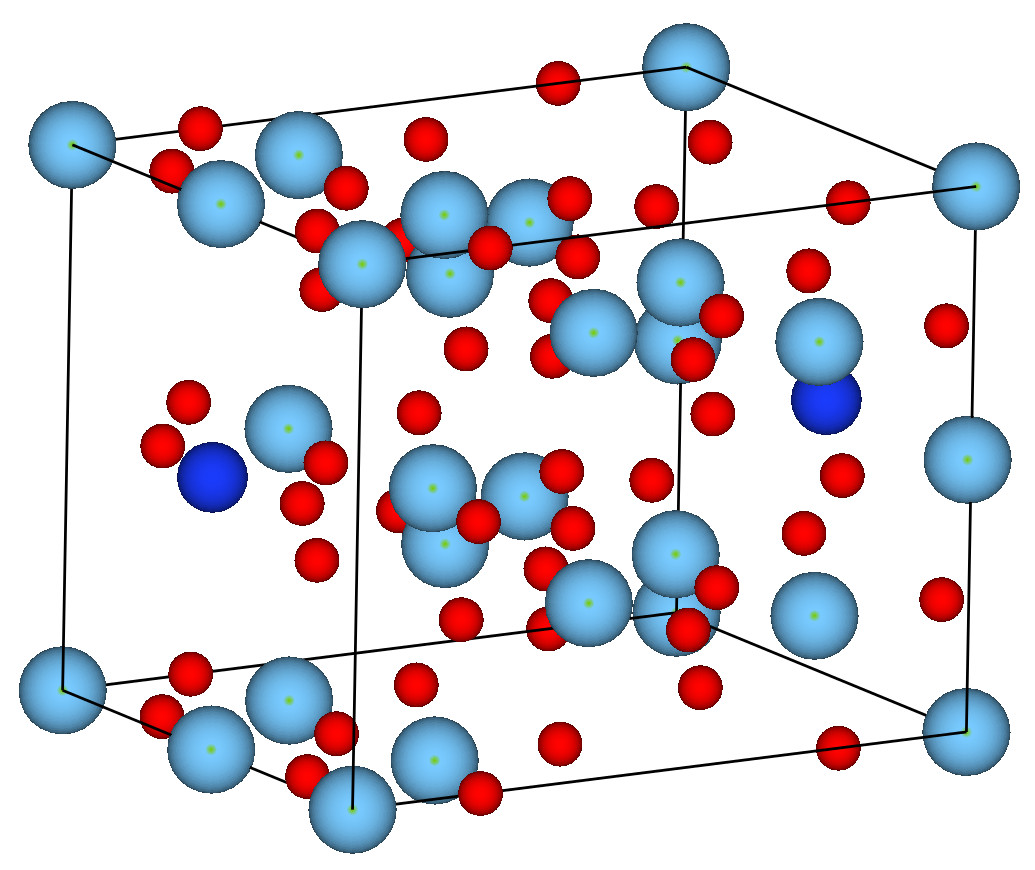
\includegraphics[width=0.9\linewidth]{figures/cell.jpg}
	\end{figure}

    \column{.6\textwidth}

    \begin{figure}
	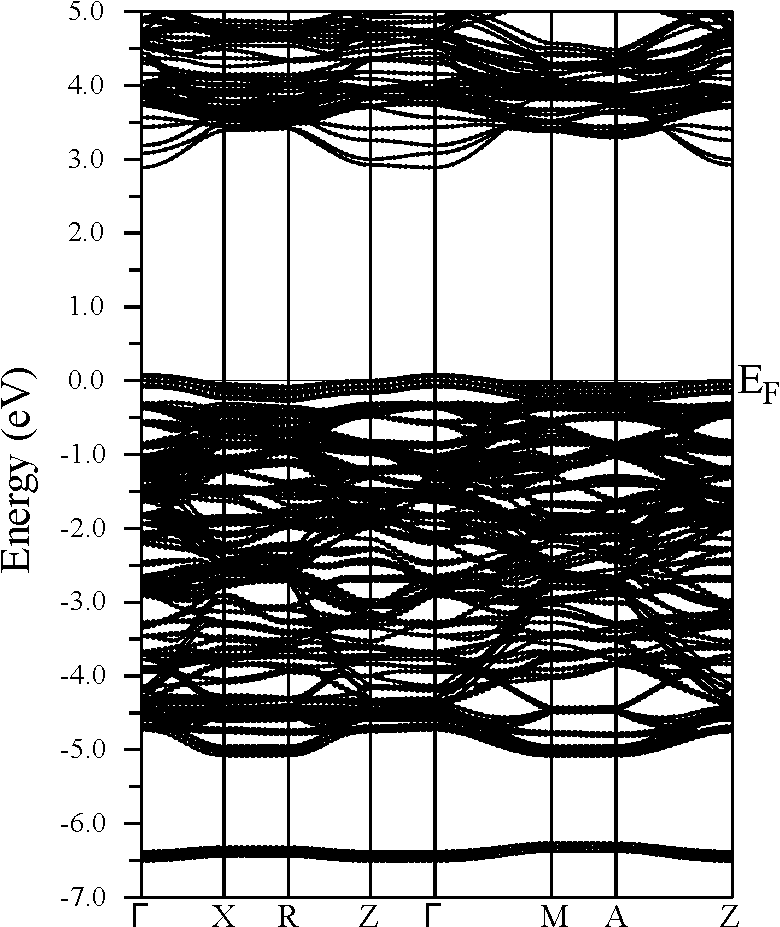
\includegraphics[height=4cm]{figures/spaghettiOSi.pdf}
	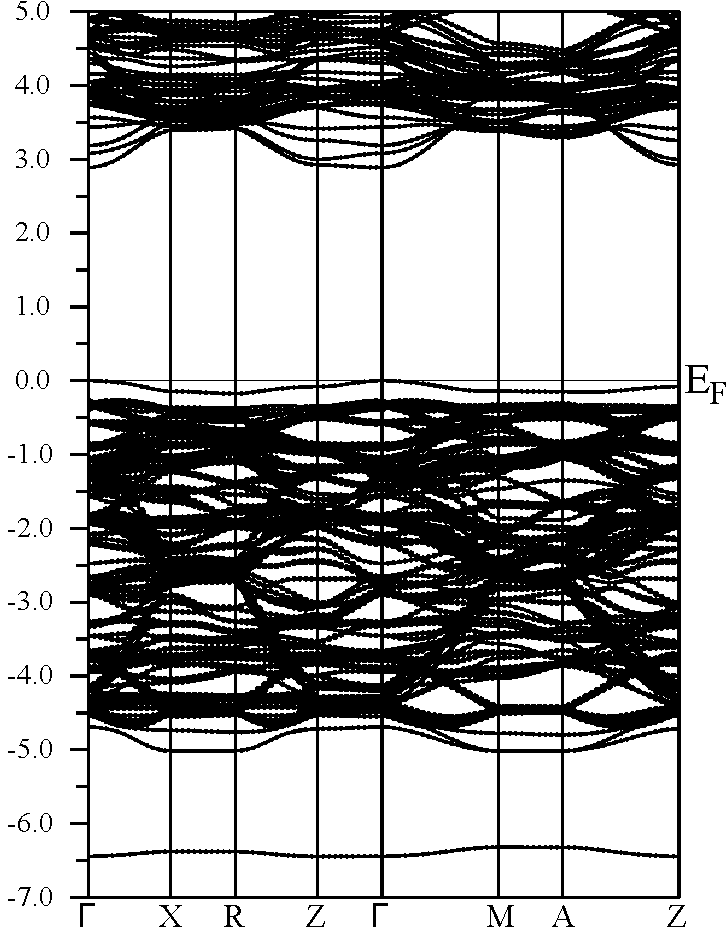
\includegraphics[height=4cm]{figures/spaghettinotOSi.pdf}
	\end{figure}

    \end{columns}

\end{frame}


\section{Conclusion}

\begin{frame}
    \frametitle{What I'm I doing at the moment?}
    \framesubtitle{Quick overview}

	\begin{itemize}
	\item IT4I project - Optical properties of TiO2 based alloys from first principle calculations (104k corehours, still almost 50\,\% left)

	\item HfO$_2$ - mBJ results for cubic, tetragonal, monoclinic and 96 atoms large amorphous cells ready, more literature search needed

	\item amorphous TiO$_2$ and Si$_x$Ti$_{1-x}$O$_2$ - WIP

	\item ,,exciting'' - a GPL DFT code with Bethe-Salpeter-equation implementation

	\item single atoms calculation - may be a way to get correct sumrule, doesn't converge ATM

	\item DLC fitting (mass density and hydrogen content from optics)

	\end{itemize}

\end{frame}

\begin{frame}
    \frametitle{Conclusion}
    \framesubtitle{Just one more minute, and its finally over}
	\begin{center}Density functional theory\end{center}
	\begin{columns}[c]
    \column{.5\textwidth}
	\begin{itemize}
	\item Can be used to calculate band gap and optical constants 

	\item Can predict optical constants of new materials

	\item Can shed some light into nature of electronic transitions

	\item Can help in development of new dispersion models
	\end{itemize}

    \column{.5\textwidth}

	\begin{itemize}
	\item ATM is not able to calculate the sum rule properly

	\item Results are worse at high energies

	\item Can calculate only direct transitions

	\end{itemize}
	\end{columns}
\end{frame}

\begin{frame}
    \frametitle{Questions}
    \framesubtitle{Everything was clear, wasn't it?}

	\begin{center}
	Thank you for your attention.
	\end{center}
	\begin{center}
	Time for questions!
	\end{center}

\end{frame}

\end{document}
